\documentclass[10pt]{article}
\usepackage[utf8]{inputenc}
\usepackage[T1]{fontenc}
\usepackage{amsmath}
\usepackage{amsfonts}
\usepackage{amssymb}
\usepackage[version=4]{mhchem}
\usepackage{stmaryrd}
\usepackage{graphicx}
\usepackage[export]{adjustbox}
\graphicspath{ {./images/} }
\usepackage{bbold}

\begin{document}
\section*{MATHEMATICS}
\section*{SECTION-A}
\begin{enumerate}
  \setcounter{enumi}{60}
  \item The distance of the point \((7,-3,-4)\) from the plane passing through the points \((2,-3,1),(-1,1,-2)\) and \((3,-4,2)\) is :\\
(1) 4\\
(2) 5\\
(3) \(5 \sqrt{2}\)\\
(4) \(4 \sqrt{2}\)
\end{enumerate}

Official Ans. by NTA (3)\\
Allen Ans. (3)\\
Sol. Equation of Plane is\\
\(=\left|\begin{array}{ccc}x-2 & y+3 & z-1 \\ -3 & 4 & -3 \\ 4 & -5 & 4\end{array}\right|=0\)\\
\(\mathrm{x}-\mathrm{z}-1=0\)\\
Distance of \(\mathrm{P}(7,-3,-4)\) from Plane is\\
\(\mathrm{d}=\left|\frac{7+4-1}{\sqrt{2}}\right|=5 \sqrt{2}\)\\
62. \(\lim _{\mathrm{t} \rightarrow 0}\left(1^{\frac{1}{\sin ^{2} \mathrm{t}}}+2^{\frac{1}{\sin ^{2} \mathrm{t}}}+\ldots .+\mathrm{n}^{\frac{1}{\sin ^{2} \mathrm{t}}}\right)^{\sin ^{2} \mathrm{t}}\) is equal to\\
(1) \(n^{2}+n\)\\
(2) \(n\)\\
(3) \(\frac{n(n+1)}{2}\)\\
(4) \(n^{2}\)

Official Ans. by NTA (2)\\
Allen Ans. (2)\\
Sol. \(\lim _{\mathrm{t} \rightarrow 0}\left(1^{\operatorname{cosec}^{2} \mathrm{t}}+2^{\operatorname{cosec}^{2} \mathrm{t}}+\ldots \ldots . .+\mathrm{n}^{\operatorname{cosec}^{2} \mathrm{t}}\right)^{\sin ^{2} \mathrm{t}} =\lim _{\mathrm{t} \rightarrow 0} \mathrm{n}\left(\left(\frac{1}{\mathrm{n}}\right)^{\operatorname{cosec}^{2} \mathrm{t}}+\left(\frac{2}{\mathrm{n}}\right)^{\operatorname{cosec}^{2} \mathrm{t}}+\ldots \ldots . .+1\right)^{\sin ^{2} \mathrm{t}} =\mathrm{n}\)

\section*{TEST PAPER WITH SOLUTION}
\begin{enumerate}
  \setcounter{enumi}{62}
  \item Let \(\overrightarrow{\mathrm{u}}=\hat{\mathrm{i}}-\hat{\mathrm{j}}-2 \mathrm{k}, \overrightarrow{\mathrm{v}}=2 \hat{\mathrm{i}}+\hat{\mathrm{j}}-\mathrm{k}, \overrightarrow{\mathrm{v}} \cdot \overrightarrow{\mathrm{w}}=2\) and \(\overrightarrow{\mathrm{v}} \times \overrightarrow{\mathrm{w}}=\overrightarrow{\mathrm{u}}+\lambda \overrightarrow{\mathrm{v}}\). Then \(\overrightarrow{\mathrm{u}} \cdot \overrightarrow{\mathrm{w}}\) is equal to\\
(1) 1\\
(2) \(\frac{3}{2}\)\\
(3) 2\\
(4) \(-\frac{2}{3}\)
\end{enumerate}

Official Ans. by NTA (1)\\
Allen Ans. (1)\\
Sol. \(\quad \overrightarrow{\mathrm{u}}=(1,-1,-2), \overrightarrow{\mathrm{v}}=(2,1,-1), \overrightarrow{\mathrm{v}} \cdot \overrightarrow{\mathrm{w}}=2\)\\
\(\overrightarrow{\mathrm{v}} \times \overrightarrow{\mathrm{w}}=\overrightarrow{\mathrm{u}}+\lambda \overrightarrow{\mathrm{v}}\)

Taking dot with \(\overrightarrow{\mathrm{W}}\) in (1)\\
\(\overrightarrow{\mathrm{w}} \cdot(\overrightarrow{\mathrm{v}} \times \overrightarrow{\mathrm{w}})=\overrightarrow{\mathrm{u}} \cdot \overrightarrow{\mathrm{w}}+\lambda \overrightarrow{\mathrm{v}} \cdot \overrightarrow{\mathrm{w}}\)\\
\(\Rightarrow 0=\overrightarrow{\mathrm{u}} \cdot \overrightarrow{\mathrm{w}}+2 \lambda\)\\
Taking dot with \(\overrightarrow{\mathrm{v}}\) in (1)\\
\(\overrightarrow{\mathrm{v}} \cdot(\overrightarrow{\mathrm{v}} \times \overrightarrow{\mathrm{w}})=\overrightarrow{\mathrm{u}} \cdot \overrightarrow{\mathrm{v}}+\lambda \overrightarrow{\mathrm{v}} \cdot \overrightarrow{\mathrm{v}}\)\\
\(\Rightarrow 0=(2-1+2)+\lambda(6)\)\\
\(\lambda=-\frac{1}{2}\)\\
\(\Rightarrow \overrightarrow{\mathrm{u}} \cdot \overrightarrow{\mathrm{w}}=-2 \lambda=1\)\\
64. The value \(\sum_{\mathrm{r}=0}^{22}{ }^{22} \mathrm{C}_{\mathrm{r}}{ }^{23} \mathrm{C}_{\mathrm{r}}\) is\\
(1) \({ }^{45} \mathrm{C}_{23}\)\\
(2) \({ }^{44} \mathrm{C}_{23}\)\\
(3) \({ }^{45} \mathrm{C}_{24}\)\\
(4) \({ }^{44} \mathrm{C}_{22}\)

Official Ans. by NTA (1)\\
Allen Ans. (1)\\
Sol. \(\sum_{\mathrm{r}=0}^{22}{ }^{22} \mathrm{C}_{\mathrm{r}} \cdot{ }^{23} \mathrm{C}_{\mathrm{r}}=\sum_{\mathrm{r}=0}^{22}{ }^{22} \mathrm{C}_{\mathrm{r}} \cdot{ }^{23} \mathrm{C}_{23-\mathrm{r}}\)\\
\(={ }^{45} \mathrm{C}_{23}\)\\
65. Let a tangent to the curve \(\mathrm{y}^{2}=24 \mathrm{x}\) meet the curve \(\mathrm{xy}=2\) at the points A and B . Then the mid points of such line segments AB lie on a parabola with the\\
(1) directrix \(4 x=3\)\\
(2) directrix \(4 x=-3\)\\
(3) Length of latus rectum \(\frac{3}{2}\)\\
(4) Length of latus rectum 2

\section*{Official Ans. by NTA (1)}
Allen Ans. (1)\\
Sol. \(y^{2}=24 x\)\\
\(\mathrm{a}=6\)\\
xy \(=2\)\\
\(\mathrm{AB} \equiv \mathrm{ty}=\mathrm{x}+6 \mathrm{t}^{2}\)\\
\(\mathrm{AB} \equiv \mathrm{T}=\mathrm{S}_{1}\)\\
\(\mathrm{kx}+\mathrm{hy}=2 \mathrm{hk}\)

From (1) and (2)\\
\(\frac{\mathrm{k}}{1}=\frac{\mathrm{h}}{-\mathrm{t}}=\frac{2 \mathrm{hk}}{-6 \mathrm{t}^{2}}\)\\
\(\Rightarrow\) then locus is \(\mathrm{y}^{2}=-3 \mathrm{x}\)\\
Therefore directrix is \(4 \mathrm{x}=3\)\\
66. Let N denote the number that turns up when a fair die is rolled. If the probability that the system of equations\\
\(\mathrm{x}+\mathrm{y}+\mathrm{z}=1\)\\
\(2 \mathrm{x}+\mathrm{Ny}+2 \mathrm{z}=2\)\\
\(3 \mathrm{x}+3 \mathrm{y}+\mathrm{Nz}=3\)\\
has unique solution is \(\frac{k}{6}\), then the sum of value of k and all possible values of N is\\
(1) 18\\
(2) 19\\
(3) 20\\
(4) 21

Official Ans. by NTA (3 )\\
Allen Ans. (3)\\
Sol. \(x+y+z=1\)\\
\(2 \mathrm{x}+\mathrm{Ny}+2 \mathrm{z}=2\)\\
\(3 \mathrm{x}+3 \mathrm{y}+\mathrm{Nz}=3\)\\
\(\Delta=\left|\begin{array}{ccc}1 & 1 & 1 \\ 2 & \mathrm{~N} & 2 \\ 3 & 3 & \mathrm{~N}\end{array}\right|\)\\
\(=(\mathrm{N}-2)(\mathrm{N}-3)\)\\
For unique solution \(\Delta \neq 0\)\\
So \(\mathrm{N} \neq 2,3\)\\
\(\Rightarrow P(\) system has unique solution \()=\frac{4}{6}\)\\
So \(\mathrm{k}=4\)\\
Therefore sum \(=4+1+4+5+6=20\)\\
67. \(\tan ^{-1}\left(\frac{1+\sqrt{3}}{3+\sqrt{3}}\right)+\sec ^{-1}\left(\sqrt{\frac{8+4 \sqrt{3}}{6+3 \sqrt{3}}}\right)\) is equal to\\
(1) \(\frac{\pi}{4}\)\\
(2) \(\frac{\pi}{2}\)\\
(3) \(\frac{\pi}{3}\)\\
(4) \(\frac{\pi}{6}\)

Official Ans. by NTA (3)\\
Allen Ans. (3)\\
Sol. \(\tan ^{-1}\left(\frac{1+\sqrt{3}}{3+\sqrt{3}}\right)+\sec ^{-1}\left(\sqrt{\frac{8+4 \sqrt{3}}{6+3 \sqrt{3}}}\right)\)\\
\(=\tan ^{-1}\left(\frac{1}{\sqrt{3}}\right)+\sec ^{-1}\left(\frac{2}{\sqrt{3}}\right)=\frac{\pi}{3}\)\\
68. Let PQR be a triangle. The points \(\mathrm{A}, \mathrm{B}\) and C are on the sides \(\mathrm{QR}, \mathrm{RP}\) and PQ respectively such that \(\frac{\mathrm{QA}}{\mathrm{AR}}=\frac{\mathrm{RB}}{\mathrm{BP}}=\frac{\mathrm{PC}}{\mathrm{CQ}}=\frac{1}{2}\). Then \(\frac{\operatorname{Area}(\triangle \mathrm{PQR})}{\operatorname{Area}(\triangle \mathrm{ABC})}\) is equal to\\
(1) 4\\
(2) 3\\
(3) 2\\
(4) \(\frac{5}{2}\)

Official Ans. by NTA (2)\\
Allen Ans. (2)\\
Sol. Let \(P\) is \(\overrightarrow{0}\), \(Q\) is \(\vec{q}\) and \(R\) is \(\vec{r}\)\\
\(A\) is \(\frac{2 \vec{q}+\vec{r}}{3}\), B is \(\frac{2 \vec{r}}{3}\) and C is \(\frac{\vec{q}}{3}\)\\
Area of \(\triangle \mathrm{PQR}\) is \(=\frac{1}{2}|\overrightarrow{\mathrm{q}} \times \overrightarrow{\mathrm{r}}|\)\\
Area of \(\Delta \mathrm{ABC}\) is \(\frac{1}{2}|\overrightarrow{\mathrm{AB}} \times \overrightarrow{\mathrm{AC}}|\)\\
\(\overrightarrow{\mathrm{AB}}=\frac{\overrightarrow{\mathrm{r}}-2 \overrightarrow{\mathrm{q}}}{3}, \overrightarrow{\mathrm{AC}}=\frac{-\overrightarrow{\mathrm{r}}-\overrightarrow{\mathrm{q}}}{3}\)\\
Area of \(\triangle \mathrm{ABC}=\frac{1}{6}|\overrightarrow{\mathrm{q}} \times \overrightarrow{\mathrm{r}}|\)\\
\(\frac{\operatorname{Area}(\triangle \mathrm{PQR})}{\operatorname{Area}(\triangle \mathrm{ABC})}=3\)\\
69. If A and B are two non-zero \(\mathrm{n} \times \mathrm{n}\) matrics such that \(A^{2}+B=A^{2} B\), then\\
(1) \(\mathrm{AB}=\mathrm{I}\)\\
(2) \(A^{2} B=I\)\\
(3) \(A^{2}=I\) or \(B=I\)\\
(4) \(A^{2} B=B A^{2}\)

Official Ans. by NTA (4 )\\
Allen Ans. (4)

Sol. \(\mathrm{A}^{2}+\mathrm{B}=\mathrm{A}^{2} \mathrm{~B}\)

\[
\left(\mathrm{A}^{2}-\mathrm{I}\right)(\mathrm{B}-\mathrm{I})=\mathrm{I}
\]

\(\mathrm{A}^{2}+\mathrm{B}=\mathrm{A}^{2} \mathrm{~B}\)\\
\(A^{2}(B-I)=B\)\\
\(\mathrm{A}^{2}=\mathrm{B}(\mathrm{B}-\mathrm{I})^{-1}\)\\
\(\mathrm{A}^{2}=\mathrm{B}\left(\mathrm{A}^{2}-\mathrm{I}\right)\)\\
\(\mathrm{A}^{2}=\mathrm{BA}^{2}-\mathrm{B}\)\\
\(\mathrm{A}^{2}+\mathrm{B}=\mathrm{BA}^{2}\)\\
\(\mathrm{A}^{2} \mathrm{~B}=\mathrm{BA}^{2}\)\\
70. Let \(y=y(x)\) be the solution of the differential equation \(x^{3} d y+(x y-1) d x=0, x>0\), \(y\left(\frac{1}{2}\right)=3-e\). Then \(y(1)\) is equal to\\
(1) 1\\
(2) e\\
(3) \(2-\mathrm{e}\)\\
(4) 3

Official Ans. by NTA (1)\\
Allen Ans. (1)\\
Sol. \(\frac{\mathrm{dy}}{\mathrm{dx}}=\frac{1-\mathrm{xy}}{\mathrm{x}^{3}}=\frac{1}{\mathrm{x}^{3}}-\frac{\mathrm{y}}{\mathrm{x}^{2}}\)\\
\(\frac{d y}{d x}+\frac{y}{x^{2}}=\frac{1}{x^{3}}\)\\
If \(=\mathrm{e}^{\int \frac{1}{\mathrm{x}^{2}} \mathrm{dx}}=\mathrm{e}^{-\frac{1}{\mathrm{x}}}\)\\
\(y \cdot e^{-\frac{1}{x}}=\int e^{-\frac{1}{x}} \cdot \frac{1}{x^{3}} d x\left(\right.\) put \(\left.-\frac{1}{x}=t\right)\)\\
\(y . e^{-\frac{1}{x}}=-\int e^{t} . t d t\)\\
\(\mathrm{y}=\frac{1}{\mathrm{x}}+1+\mathrm{Ce}^{\frac{1}{\mathrm{x}}}\)\\
Where C is constant\\
Put \(\mathrm{x}=\frac{1}{2}\)\\
\(3-\mathrm{e}=2+1+\mathrm{Ce}^{2}\)\\
\(\mathrm{C}=-\frac{1}{\mathrm{e}}\)\\
\(y(1)=1\)\\
71. The area enclosed by the curves \(y^{2}+4 x=4\) and \(\mathrm{y}-2 \mathrm{x}=2\) is :\\
(1) \(\frac{25}{3}\)\\
(2) \(\frac{22}{3}\)\\
(3) 9\\
(4) \(\frac{23}{3}\)

\section*{Official Ans. by NTA (3)}
\section*{Allen Ans. (3)}
Sol.\\
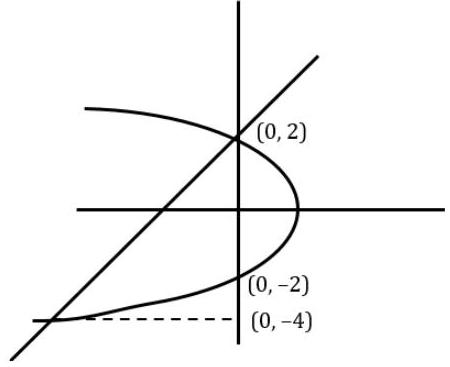
\includegraphics[max width=\textwidth, center]{2025_10_03_68ad1a1a030f3f6076e9g-3}\\
\(\mathrm{y}^{2}+4 \mathrm{x}=4\)\\
\(y^{2}=-4(x-1)\)\\
\(\mathrm{A}=\int_{-4}^{2}\left(\frac{4-\mathrm{y}^{2}}{4}-\frac{\mathrm{y}-2}{2}\right) \mathrm{dy}=9\)\\
72. Let \(\alpha\) be a root of the equation\\
\((\mathrm{a}-\mathrm{c}) \mathrm{x}^{2}+(\mathrm{b}-\mathrm{a}) \mathrm{x}+(\mathrm{c}-\mathrm{b})=0\) where \(\mathrm{a}, \mathrm{b}, \mathrm{c}\) are distinct real numbers such that the matrix\\
\(\left[\begin{array}{ccc}\alpha^{2} & \alpha & 1 \\ 1 & 1 & 1 \\ a & b & c\end{array}\right]\)\\
is singular. Then the value of\\
\(\frac{(a-c)^{2}}{(b-a)(c-b)}+\frac{(b-a)^{2}}{(a-c)(c-b)}+\frac{(c-b)^{2}}{(a-c)(b-a)}\) is\\
(1) 6\\
(2) 3\\
(3) 9\\
(4) 12

\section*{Official Ans. by NTA (2 )}
\section*{Allen Ans. (2)}
Sol. \(\quad \Delta=0=\left|\begin{array}{ccc}\alpha^{2} & \alpha & 1 \\ 1 & 1 & 1 \\ \mathrm{a} & \mathrm{b} & \mathrm{c}\end{array}\right|\)\\
\(\Rightarrow \alpha^{2}(\mathrm{c}-\mathrm{b})-\alpha(\mathrm{c}-\mathrm{a})+(\mathrm{b}-\mathrm{a})=0\)\\
It is singular when \(\alpha=1\)\\
\(\frac{(a-c)^{2}}{(b-a)(c-b)}+\frac{(b-a)^{2}}{(a-c)(c-b)}+\frac{(c-b)^{2}}{(a-c)(b-a)}\)\\
\(\frac{(a-b)^{3}+(b-c)^{3}+(c-a)^{3}}{(a-b)(b-c)(c-a)}\)\\
\(=3 \frac{(a-b)(b-c)(c-a)}{(a-b)(b-c)(c-a)}=3\)\\
73. The distance of the point \((-1,9,-16)\) from the plane \(2 \mathrm{x}+3 \mathrm{y}-\mathrm{z}=5\) measured parallel to the line \(\frac{x+4}{3}=\frac{2-y}{4}=\frac{z-3}{12}\) is\\
(1) \(13 \sqrt{2}\)\\
(2) 31\\
(3) 26\\
(4) \(20 \sqrt{2}\)

Official Ans. by NTA (3 )\\
Allen Ans. (3)\\
Sol. Equation of line\\
\(\frac{\mathrm{x}+1}{3}=\frac{\mathrm{y}-9}{-4}=\frac{\mathrm{z}+16}{12}\)\\
G.P on line \((3 \lambda-1,-4 \lambda+9,12 \lambda-16)\)\\
point of intersection of line \& plane\\
\(6 \lambda-2-12 \lambda+27-12 \lambda+16=5\)\\
\(\lambda=2\)\\
Point (5, 1, 8)\\
Distance \(=\sqrt{36+64+576}=26\)\\
74. For three positive integers \(p, q, r, x^{p q^{2}}=y^{q r}=z^{p^{2} r}\) and \(r=p q+1\) such that \(3,3 \log _{y} x, 3 \log _{z} y, 7 \log _{x} z\) are in A.P. with common difference \(\frac{1}{2}\). Then \(r-p-q\) is equal to\\
(1) 2\\
(2) 6\\
(3) 12\\
(4) -6

Official Ans. by NTA (1)\\
Allen Ans. (1)\\
Sol. \(\mathrm{pq}^{2}=\log _{\mathrm{x}} \lambda\)\\
\(\mathrm{qr}=\log _{\mathrm{y}} \lambda\)\\
\(\mathrm{p}^{2} \mathrm{r}=\log _{\mathrm{z}} \lambda\)\\
\(\log _{y} x=\frac{q r}{p q^{2}}=\frac{r}{p q}\)\\
\(\log _{x} z=\frac{p q^{2}}{p^{2} r}=\frac{q^{2}}{p r}\)\\
\(\log _{z} y=\frac{p^{2} r}{q r}=\frac{p^{2}}{q}\)\\
\(3, \frac{3 r}{p q}, \frac{3 p^{2}}{q}, \frac{7 q^{2}}{p r}\) in A.P\\
\(\frac{3 \mathrm{r}}{\mathrm{pq}}-3=\frac{1}{2}\)\\
\(\mathrm{r}=\frac{7}{6} \mathrm{pq}\) \(\_\_\_\_\) (4)\\
\(\mathrm{r}=\mathrm{pq}+1\)\\
\(\mathrm{pq}=6\) \(\_\_\_\_\)\\
\(\mathrm{r}=7\)\\
\(\frac{3 \mathrm{p}^{2}}{\mathrm{q}}=4\)\\
After solving \(\mathrm{p}=2\) and \(\mathrm{q}=3\)\\
75. Let\\
\(\mathrm{p}, \mathrm{q} \in \mathbb{R}\) and \((1-\sqrt{3} \mathrm{i})^{200}=2^{199}(\mathrm{p}+\mathrm{iq})\), \(\mathrm{i}=\sqrt{-1}\) Then \(\mathrm{p}+\mathrm{q}+\mathrm{q}^{2}\) and \(\mathrm{p}-\mathrm{q}+\mathrm{q}^{2}\) are roots of the equation.\\
(1) \(x^{2}+4 x-1=0\)\\
(2) \(x^{2}-4 x+1=0\)\\
(3) \(x^{2}+4 x+1=0\)\\
(4) \(x^{2}-4 x-1=0\)

Official Ans. by NTA (2)\\
Allen Ans. (2)\\
Sol. \(\quad(1-\sqrt{3} \mathrm{i})^{200}=2^{199}(\mathrm{p}+\mathrm{iq})\)\\
\(2^{200}\left(\cos \frac{\pi}{3}-\mathrm{i} \sin \frac{\pi}{3}\right)^{200}=2^{199}(\mathrm{p}+\mathrm{iq})\)\\
\(2\left(-\frac{1}{2}-\mathrm{i} \frac{\sqrt{3}}{2}\right)=\mathrm{p}+\mathrm{iq}\)\\
\(\mathrm{p}=-1, \mathrm{q}=-\sqrt{3}\)\\
\(\alpha=\mathrm{p}+\mathrm{q}+\mathrm{q}^{2}=2-\sqrt{3}\)\\
\(\beta=\mathrm{p}-\mathrm{q}+\mathrm{q}^{2}=2+\sqrt{3}\)\\
\(\alpha+\beta=4\)\\
\(\alpha \cdot \beta=1\)\\
equation \(\mathrm{x}^{2}-4 \mathrm{x}+1=0\)\\
76. The relation \(\mathrm{R}=\{(\mathrm{a}, \mathrm{b}): \operatorname{gcd}(\mathrm{a}, \mathrm{b})=1,2 \mathrm{a} \neq \mathrm{b}, \mathrm{a}, \mathrm{b} \in \mathbb{Z}\}\) is: \(\_\_\_\_\)\\
(1) transitive but not reflexive\\
(2) symmetric but not transitive\\
(3) reflexive but not symmetric\\
(4) neither symmetric nor transitive

Official Ans. by NTA (4)\\
Allen Ans. (4)\\
Sol. Reflexive : \((\mathrm{a}, \mathrm{a}) \Rightarrow \operatorname{gcd}\) of \((\mathrm{a}, \mathrm{a})=1\)\\
Which is not true for every a \(\epsilon Z\).\\
Symmetric:\\
Take \(\mathrm{a}=2, \mathrm{~b}=1 \Rightarrow \operatorname{gcd}(2,1)=1\)\\
Also \(2 \mathrm{a}=4 \neq \mathrm{b}\)\\
Now when \(\mathrm{a}=1, \mathrm{~b}=2 \Rightarrow \operatorname{gcd}(1,2)=1\)\\
Also now \(2 \mathrm{a}=2=\mathrm{b}\)\\
Hence \(\mathrm{a}=2 \mathrm{~b}\)

\section*{\(\Rightarrow \mathrm{R}\) is not Symmetric}
Transitive:\\
Let \(\mathrm{a}=14, \mathrm{~b}=19, \mathrm{c}=21\)\\
\(\operatorname{gcd}(\mathrm{a}, \mathrm{b})=1\)\\
\(\operatorname{gcd}(\mathrm{b}, \mathrm{c})=1\)\\
\(\operatorname{gcd}(\mathrm{a}, \mathrm{c})=7\)\\
Hence not transitive\\
\(\Rightarrow R\) is neither symmetric nor transitive.\\
77. The compound statement\\
\((\sim(\mathrm{P} \wedge \mathrm{Q})) \vee((\sim \mathrm{P}) \wedge \mathrm{Q}) \Rightarrow((\sim \mathrm{P}) \wedge(\sim \mathrm{Q}))\) is equivalent to\\
(1) \(((\sim P) \vee Q) \wedge((\sim Q) \vee P)\)\\
(2) \((\sim\) Q \() \vee\) P\\
(3) \(((\sim P) \vee Q) \wedge(\sim Q)\)\\
(4) \((\sim P) \vee Q\)

Official Ans. by NTA (1)\\
Allen Ans. (1)\\
Sol. Let \(\mathbf{r}=(\sim(\mathrm{P} \wedge \mathrm{Q})) \vee((\sim \mathrm{P}) \wedge \mathrm{Q}) ; \quad \mathrm{s}= ((\sim \mathrm{P}) \wedge(\sim \mathrm{Q}))\)

\begin{center}
\begin{tabular}{|l|l|l|l|l|l|l|}
\hline
P & Q & \(\sim(\mathrm{P} \wedge \mathrm{Q})\) & \((-\mathrm{P}) \wedge \mathrm{Q}\) & r & s & \(\mathrm{r} \rightarrow \mathrm{s}\) \\
\hline
T & T & F & F & F & F & T \\
\hline
T & F & T & F & T & F & F \\
\hline
F & T & T & T & T & F & F \\
\hline
F & F & T & F & T & T & T \\
\hline
\end{tabular}
\end{center}

Option (A) : \(((\sim \mathrm{P}) \vee \mathrm{Q}) \wedge((\sim \mathrm{Q}) \vee \mathrm{P})\)\\
is equivalent to (not of only P\() \wedge(\) not of only Q\() =(\) Both \(\mathrm{P}, \mathrm{Q})\) and (neither P nor Q )\\
78. Let \(f(x)=\left\{\begin{array}{cl}x^{2} \sin \left(\frac{1}{x}\right) & , x \neq 0 \\ 0 & , x=0\end{array}\right.\); Then at \(x=0\)\\
(1) \(f\) is continuous but not differentiable\\
(2) \(f\) is continuous but \(f^{\prime}\) is not continuous\\
(3) f and \(\mathrm{f}^{\prime}\) both are continuous\\
(4) \(\mathrm{f}^{\prime}\) is continuous but not differentiable

Official Ans. by NTA (2)\\
Allen Ans. (2)

Sol. Continuity of \(\mathrm{f}(\mathrm{x}): \mathrm{f}\left(0^{+}\right)=\mathrm{h}^{2} \cdot \sin \frac{1}{\mathrm{~h}}=0\)\\
\(f\left(0^{-}\right)=(-h)^{2} \cdot \sin \left(\frac{-1}{h}\right)=0\)\\
\(\mathrm{f}(0)=0\)\\
\(\mathrm{f}(\mathrm{x})\) is continuous\\
\(f^{\prime}\left(0^{+}\right)=\lim _{h \rightarrow 0} \frac{f(0+h)-f(0)}{h}=\frac{h^{2} \cdot \sin \left(\frac{1}{h}\right)-0}{h}=0\)\\
\(f^{\prime}\left(0^{-}\right)=\lim _{h \rightarrow 0} \frac{f(0-h)-f(0)}{-h}=\frac{h^{2} \cdot \sin \left(\frac{1}{-h}\right)-0}{-h}=0\)\\
\(\mathrm{f}(\mathrm{x})\) is differentiable.\\
\(f^{\prime}(x)=2 x \cdot \sin \left(\frac{1}{x}\right)+x^{2} \cdot \cos \left(\frac{1}{x}\right) \cdot \frac{-1}{x^{2}}\)\\
\(f^{\prime}(x)=\left\{\begin{array}{cl}2 x \cdot \sin \left(\frac{1}{x}\right)-\cos \left(\frac{1}{x}\right), & x \neq 0 \\ 0, & x=0\end{array}\right.\)\\
\(\Rightarrow \mathrm{f}^{\prime}(\mathrm{x})\) is not continuous (as \(\cos \left(\frac{1}{\mathrm{x}}\right)\) is highly oscillating at \(\mathrm{x}=0\) )\\
79. The equation \(x^{2}-4 x+[x]+3=x[x]\), where \([x]\) denotes the greatest integer function, has:\\
(1) exactly two solutions in \((-\infty, \infty)\)\\
(2) no solution\\
(3) a unique solution in \((-\infty, 1)\)\\
(4) a unique solution in \((-\infty, \infty)\)

Official Ans. by NTA (4 )\\
Allen Ans. (4)\\
Sol. \(\quad x^{2}-4 x+[x]+3=x[x]\)\\
\(\Rightarrow \mathrm{x}^{2}-4 \mathrm{x}+3=\mathrm{x}[\mathrm{x}]-[\mathrm{x}]\)\\
\(\Rightarrow(\mathrm{x}-1)(\mathrm{x}-3)=[\mathrm{x}] .(\mathrm{x}-1)\)\\
\(\Rightarrow \mathrm{x}=1\) or \(\mathrm{x}-3=[\mathrm{x}]\)\\
\(\Rightarrow \mathrm{x}-[\mathrm{x}]=3\)\\
\(\Rightarrow\{\mathrm{x}\}=3\) (Not Possible)\\
Only one solution \(x=1\) in \((-\infty, \infty)\)\\
80. Let \(\Omega\) be the sample space and \(\mathrm{A} \subseteq \Omega\) be an event. Given below are two statements :\\
(S1) : If \(\mathrm{P}(\mathrm{A})=0\), then \(\mathrm{A}=\phi\)\\
(S2) : If \(\mathrm{P}(\mathrm{A})=\), then \(\mathrm{A}=\Omega\)\\
Then\\
(1) only (S1) is true\\
(2) only (S2) is true\\
(3) both (S1) and (S2) are true\\
(4) both (S1) and (S2) are false

Official Ans. by NTA (4)\\
Allen Ans. (3)

Sol. \(\Omega=\) sample space\\
\(\mathrm{A}=\) be an event\\
If \(\mathrm{P}(\mathrm{A})=0 \Rightarrow \mathrm{~A}=\phi\)\\
If \(\mathrm{P}(\mathrm{A})=1 \Rightarrow \mathrm{~A}=\Omega\)\\
Then both statement are true

\section*{SECTION-B}
\begin{enumerate}
  \setcounter{enumi}{80}
  \item Let C be the largest circle centred at \((2,0)\) and inscribed in the ellipse \(=\frac{x^{2}}{36}+\frac{y^{2}}{16}=1\).
\end{enumerate}

If \((1, \alpha)\) lies on C , then \(10 \alpha^{2}\) is equal to \(\_\_\_\_\)\\
Official Ans. by NTA (118)\\
Allen Ans. (118)\\
Sol.\\
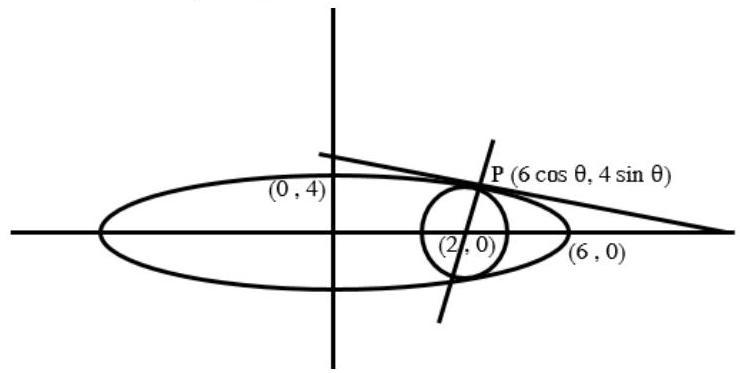
\includegraphics[max width=\textwidth, center]{2025_10_03_68ad1a1a030f3f6076e9g-6}

Equation of normal of ellipse \(\frac{x^{2}}{36}+\frac{y^{2}}{16}=1\) at any point \(\mathrm{P}(6 \cos \theta, 4 \sin \theta)\) is\\
\(3 \sec \theta x-2 \operatorname{cosec} \theta y=10\) this normal is also the normal of the circle passing through the point \((2,0)\) So,\\
\(6 \sec \theta=10\) or \(\sin \theta=0\) (Not possible)\\
\(\cos \theta=\frac{3}{5}\) and \(\sin \theta=\frac{4}{5}\) so point \(\mathrm{P}=\left(\frac{18}{5}, \frac{16}{5}\right)\)\\
So the largest radius of circle\\
\(r=\frac{\sqrt{320}}{5}\)\\
So the equation of circle \((x-2)^{2}+y^{2}=\frac{64}{5}\)\\
Passing it through \((1, \alpha)\)\\
Then \(\alpha^{2}=\frac{59}{5}\)\\
\(10 \alpha^{2}=118\)\\
82. Suppose \(\sum_{\mathrm{r}=0}^{2023} \mathrm{r}^{2}{ }^{2023} \mathrm{C}_{\mathrm{r}}=2023 \times \alpha \times 2^{2022}\). Then the value of \(\alpha\) is \(\_\_\_\_\)\\
Official Ans. by NTA (1012)\\
Allen Ans. (1012)

Sol. using result\\
\(\sum_{\mathrm{r}=0}^{\mathrm{n}} \mathrm{r}^{2}{ }^{\mathrm{n}} \mathrm{C}_{\mathrm{r}}=\mathrm{n}(\mathrm{n}+1) \cdot 2^{\mathrm{n}-2}\)

Then \(\sum_{\mathrm{r}=0}^{2023} \mathrm{r}^{2}{ }^{2023} \mathrm{C}_{\mathrm{r}}=2023 \times 2024 \times 2^{2021}\)\\
\(=2023 \times \alpha \times 2^{2022}\) So,\\
\(\Rightarrow \alpha=1012\)\\
83. The value of \(12 \int_{0}^{3}\left|\mathrm{x}^{2}-3 \mathrm{x}+2\right| \mathrm{dx}\) is \(\_\_\_\_\)

Official Ans. by NTA (22)\\
Allen Ans. (22)\\
Sol. \(\quad 12 \int_{0}^{3}\left|\mathrm{x}^{2}-3 \mathrm{x}+2\right| \mathrm{dx}\)\\
\(=12 \int_{0}^{3}\left|\left(x-\frac{3}{2}\right)^{2}-\frac{1}{4}\right| d x\)\\
If \(\mathrm{x}-\frac{3}{2}=\mathrm{t}\)\\
\(\mathrm{dx}=\mathrm{dt}\)\\
\(=24 \int_{0}^{3 / 2}\left|\mathrm{t}^{2}-\frac{1}{4}\right| \mathrm{dt}\)\\
\(=24\left[-\int_{0}^{1 / 2}\left(\mathrm{t}^{2}-\frac{1}{4}\right) \mathrm{dt}+\int_{1 / 2}^{3 / 2}\left(\mathrm{t}^{2}-\frac{1}{4}\right) \mathrm{dt}\right]=22\)\\
84. The number of 9 digit numbers, that can be formed using all the digits of the number 123412341 so that the even digits occupy only even places, is \(\_\_\_\_\)\\
Official Ans. by NTA (60)\\
Allen Ans. (60)\\
Sol. Even digits occupy at even places\\
\(\frac{4!}{2!2!} \times \frac{5!}{2!3!}=\frac{24 \times 120}{4 \times 12}=60\)\\
85. Let \(\lambda \in \mathbb{R}\) and let the equation E be \(|x|^{2}-2|x|+|\lambda-3|=0\). Then the largest element in the set \(S=\)\\
\(\{\mathrm{x}+\lambda: \mathrm{x}\) is an integer solution of E\(\}\) is \(\_\_\_\_\)\\
Official Ans. by NTA (5)\\
Allen Ans. (5)\\
Sol. \(|x|^{2}-2|x|+|\lambda-3|=0\)\\
\(|x|^{2}-2|x|+|\lambda-3|-1=0\)\\
\((|\mathrm{x}|-1)^{2}+|\lambda-3|=1\)\\
At \(\lambda=3, \mathrm{x}=0\) and 2 ,\\
at \(\lambda=4\) or 2 , then\\
\(\mathrm{x}=1\) or -1\\
So maximum value of \(\mathrm{x}+\lambda=5\)\\
86. A boy needs to select five courses from 12 available courses, out of which 5 courses are language courses. If he can choose at most two language courses, then the number of ways he can choose five courses is

Official Ans. by NTA (546)\\
Allen Ans. (546)\\
Sol. For at most two language courses\\
\(={ }^{5} \mathrm{C}_{2} \times{ }^{7} \mathrm{C}_{3}+{ }^{5} \mathrm{C}_{1} \times{ }^{7} \mathrm{C}_{4}+{ }^{7} \mathrm{C}_{5}=546\)\\
87. Let a tangent to the Curve \(9 x^{2}+16 y^{2}=144\) intersect the coordinate axes at the points A and B . Then, the minimum length of the line segment AB is \(\_\_\_\_\)\\
Official Ans. by NTA (7)\\
Allen Ans. (7)\\
Sol. Equation of tangent at point \(\mathrm{P}(4 \cos \theta, 3 \sin \theta)\) is \(\frac{x \cos \theta}{4}+\frac{y \sin \theta}{3}=1\) So \(A\) is \((4 \sec \theta, 0)\) and point B is \((0,3 \operatorname{cosec} \theta)\)\\
Length \(\mathbf{A B}=\sqrt{16 \sec ^{2} \theta+9 \operatorname{cosec}^{2} \theta}\)\\
\(=\sqrt{25+16 \tan ^{2} \theta+9 \cot ^{2} \theta} \geq 7\)\\
88. The value of \(\frac{8}{\pi} \int_{0}^{\frac{\pi}{2}} \frac{(\cos x)^{2023}}{(\sin x)^{2023}+(\cos x)^{2023}} d x\) is \(\_\_\_\_\) .

Official Ans. by NTA (2)\\
Allen Ans. (2)\\
Sol. \(I=\frac{8}{\pi} \int_{0}^{\frac{\pi}{2}} \frac{(\cos x)^{2023}}{(\sin x)^{2023}+(\cos x)^{2023}} d x\)

Using \(\int_{0}^{a} f(x) d x=\int_{0}^{a} f(a-x) d x\)\\
\(I=\frac{8}{\pi} \int_{0}^{\frac{\pi}{2}} \frac{(\sin x)^{2023}}{(\sin x)^{2023}+(\cos x)^{2023}} d x\)

Adding (1) \& (2)\\
\(2 I=\frac{8}{\pi} \int_{0}^{\frac{\pi}{2}} 1 d x\)\\
\(\mathrm{I}=2\)\\
89. The shortest distance between the lines \(\frac{x-2}{3}=\frac{y+1}{2}=\frac{z-6}{2}\) and \(\frac{x-6}{3}=\frac{1-y}{2}=\frac{z+8}{0}\) is equal to \(\_\_\_\_\)\\
Official Ans. by NTA (14)\\
Allen Ans. (14)\\
Sol. Shortest distance between the lines\\
\(=\frac{\left|\begin{array}{ccc}4 & 2 & -14 \\ 3 & 2 & 2 \\ 3 & -2 & 0\end{array}\right|}{\left.\left|\begin{array}{ccc}\hat{i} & \hat{j} & k \\ 3 & 2 & 2 \\ 3 & -2 & 0\end{array}\right| \right\rvert\,}\)\\
\(=\frac{16+12+168}{|-4 \hat{i}+6 \hat{j}-12 k|}=\frac{196}{14}=14\)\\
90. The \(4^{\text {th }}\) term of GP is 500 and its common ratio is \(\frac{1}{m}, m \in N\). Let \(S_{n}\) denote the sum of the first \(n\) terms of this GP. If \(\mathrm{S}_{6}>\mathrm{S}_{5}+1\) and \(\mathrm{S}_{7}<\mathrm{S}_{6}+\frac{1}{2}\), then the number of possible values of m is \(\_\_\_\_\)\\
Official Ans. by NTA (12)\\
Allen Ans. (12)\\
Sol. \(\mathrm{T}_{4}=500 \quad\) where \(\mathrm{a}=\) first term,

\[
\mathrm{r}=\text { common ratio }=\frac{1}{\mathrm{~m}}, \mathrm{~m} \in \mathrm{~N}
\]

\(\mathrm{ar}^{3}=500\)\\
\(\frac{\mathrm{a}}{\mathrm{m}^{3}}=500\)\\
\(\mathrm{S}_{\mathrm{n}}-\mathrm{S}_{\mathrm{n}-1}=\mathrm{ar}^{\mathrm{n}-1}\)\\
\(\mathrm{S}_{6}>\mathrm{S}_{5}+1 \quad\) and \(\mathrm{S}_{7}-\mathrm{S}_{6}<\frac{1}{2}\)\\
\(\mathrm{S}_{6}-\mathrm{S}_{5}>1 \quad \frac{\mathrm{a}}{\mathrm{m}^{6}}<\frac{1}{2}\)\\
\(\operatorname{ar}^{5}>1 \quad \mathrm{~m}^{3}>10^{3}\)\\
\(\frac{500}{\mathrm{~m}^{2}}>1\)\\
\(\mathrm{m}^{2}<500 \ldots \ldots\). (1)\\
From (1) and (2)\\
\(\mathrm{m}=11,12,13 \ldots \ldots \ldots \ldots . ., 22\)\\
So number of possible values of m is 12


\end{document}